\section{Auswertung}


\begin{figure}
	\centering
	\begin{subfigure}{0.49\linewidth}
		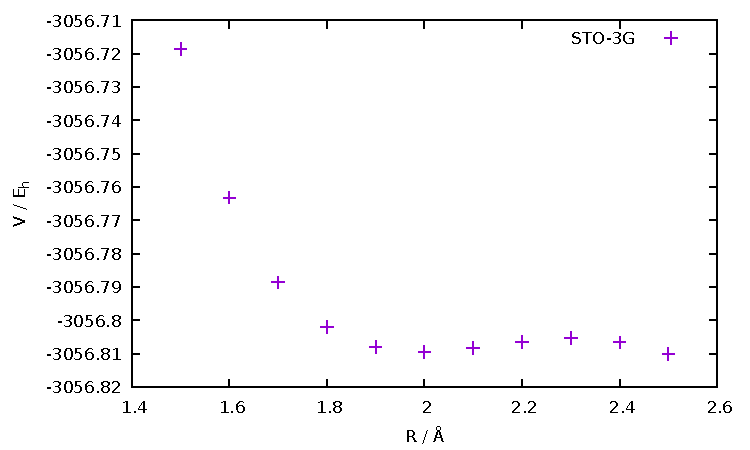
\includegraphics[width=\linewidth]{STO.pdf}
		\subcaption{Scanergebniss nach dem STO-3G Datensatz}
		\label{abb:STO}
	\end{subfigure}
	\hfill
	\begin{subfigure}{0.49\linewidth}
		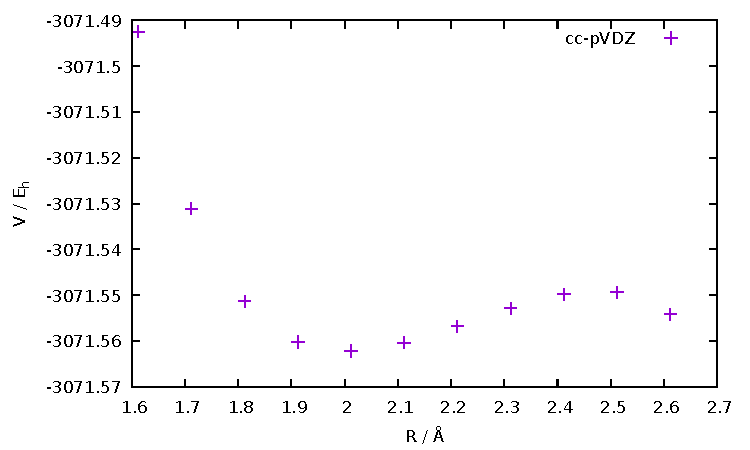
\includegraphics[width=\linewidth]{cc.pdf}
		\subcaption{Scanergebniss nach dem cc-pVDZ Datensatz}
 		\label{abb:cc}
	\end{subfigure}
	\caption{Totale Energie über Abstand der Reaktionspartner entlang der Reaktionskoordinate}
\end{figure}
Nach beenddigung der Simulationen sind die in den Abbildungen \ref{abb:STO} und \ref{abb:cc}, sowie der Tabelle \ref{tab:AusgDaten} enthaltenen Daten erhalten worden.
Wie hier Zusehen wurden als erstes nicht-SI-Einheiten in solche umgerechnet. 
Außerdem ist die Elektronische Energie mit der Avogadrozahl multipliziert worden, um später eine Molare Reaktionsenthalpie zu erhalten.
Dies vereinfacht im Weitern die Vergleichbarkeit.
Nach Gleichung \ref{eq:rktEnth} ist die Summe aus Elektrischer Energie und die Nullpunkts-Schwingungsenergie die Reaktionsenthalpie.
\begin{equation}
H=EE+ZPVE
\label{eq:rktEnth}
\end{equation}

\begin{table}{b}
\centering
\begin{tabular}{ll|cccc}
Basissatz&         				& STO-3G              & STO-3G              & Cc-pVDZ             & Cc-pVDZ\\
Zustand	 &           				& Produkt             & Übergangszustand    & Produkt             & Übergangszustand\\
\hline
\hline
EE       &/\unit{\hartree} 			& -3038,2712          & -3038,259           & -3071,575           & -3071,549\\
EE       &/\unit{\joule\per\mole}    		& -7976898112,48099   & -7976866081,71397   & -8064336330,42495   & -8064268068,13456\\
ZPVE     &/\unit{\hartree}    			& 0,044396            & 0,043806            & 0,040254            & 0,039045\\
ZPVE     &/\unit{\joule\per\mole} 		& 116560,486306063    & 115011,457408852    & 105685,778353101    & 102511,581850172\\
T        &/\unit{\kelvin}                	& 298,15              & 298,15              & 298,15              & 298,15\\
S        &/\unit{\cal\per\mole\per\kelvin}    	& 78,242              & 70,352              & 28,647              & 73,321\\
S        &/\unit{\joule\per\mole\per\kelvin}	& 327,364528          & 294,352768          & 119,859048          & 306,775064\\
\end{tabular}
\caption{Ausgangsdaten nach der Simulation der Reaktion}
\label{tab:AusgDaten}
\end{table}  

Weiter kann über die Gibbs-Gleichung (Gleichung \ref{eq:gibbs} die Gleichnamige Enthalpie (oder auch Freie Reaktionsenthalpie genannt) errechnet werden.
\begin{equation}
G=H-t\Delta s
\label{eq:gibbs}
\end{equation}
Die Differenz der Gibbs Energien zwischen Produkt und Übergangszustand, gibt die Aktivierungs Energie.
Diese Kann nun über die Arrhenius Gleichung (Gleichung \ref{eq:arr}) in die dazugehörige geschwindigkeitskonstante umgerechnet werden.
\begin{equation}
k=e^{\frac{-E_A}{R\cdot T}}
\label{eq:arr}
\end{equation}
Die Resultate dieser Rechnungen sind in Tabelle \ref{tab:res} dargestellt.
Der cc-pVDZ Basissatz ist generell größer und damit genauer.
Dies spiegelt sich zumbeispiel auch in der Rechenzeit wieder, welche hier Deutlich länger gedauert haben. 
Zusehen ist diese Tatsache unter anderem an den Geringeren Energien.
Nach dem Variationtheorem, wird davon ausgegangen, das solche simulationen stets einen zugroßen Energiewert errechnen.
Somit sind niedrigere Ergebnisse immer näher an dem wahren Wert.
Weiter ist die errechnete Aktivierungs energie Sehr nah an den Literatur Werten.

